\documentclass[10pt,a4paper,german]{scrartcl}
\usepackage[utf8]{inputenc}

\usepackage{acl2005}

\usepackage[german]{babel}
\usepackage{amsmath}
\usepackage{amsfonts}
\usepackage{amsthm}
\usepackage{amssymb}
\usepackage{graphicx}
\usepackage{lmodern}

\usepackage{units}

\usepackage{multirow}

\usepackage{hyperref}

\usepackage{listings}
\usepackage{color}

\usepackage{pgfplotstable}
\usepackage{booktabs}
\usepackage{array}
\usepackage{colortbl}


\definecolor{dkgreen}{rgb}{0,0.6,0}
\definecolor{gray}{rgb}{0.5,0.5,0.5}
\definecolor{mauve}{rgb}{0.58,0,0.82}

\lstset{ %
  language=Lua,                % the language of the code
  basicstyle=\small,           % the size of the fonts that are used for the code
  %numbers=left,                   % where to put the line-numbers
  numberstyle=\tiny\color{gray},  % the style that is used for the line-numbers
  stepnumber=2,                   % the step between two line-numbers. If it's 1, each line
                                  % will be numbered
  numbersep=5pt,                  % how far the line-numbers are from the code
  backgroundcolor=\color{white},      % choose the background color. You must add \usepackage{color}
  showspaces=false,               % show spaces adding particular underscores
  showstringspaces=false,         % underline spaces within strings
  showtabs=false,                 % show tabs within strings adding particular underscores
  %frame=single,                   % adds a frame around the code
  rulecolor=\color{black},        % if not set, the frame-color may be changed on line-breaks within not-black text (e.g. commens (green here))
  tabsize=2,                      % sets default tabsize to 2 spaces
  captionpos=b,                   % sets the caption-position to bottom
  breaklines=true,                % sets automatic line breaking
  breakatwhitespace=false,        % sets if automatic breaks should only happen at whitespace
  title=\lstname,                   % show the filename of files included with \lstinputlisting;
                                  % also try caption instead of title
  keywordstyle=\color{blue},          % keyword style
  commentstyle=\color{dkgreen},       % comment style
  stringstyle=\color{mauve},         % string literal style
  escapeinside={\%*}{*)},            % if you want to add a comment within your code
  morekeywords={*,...}               % if you want to add more keywords to the set
}


%\usepackage{trsym}
%\usepackage{dsfont}
%\usepackage{pifont}

%\usepackage{kpfonts}
%\usepackage{fourier}
%\usepackage[left=2cm,right=2cm,top=2cm,bottom=2cm]{geometry}

%\usepackage{times}
%\usepackage{latexsym}

\newcommand{\EnAmpTable}[1]{\pgfplotstabletypeset[%
				every head row/.style={%
					before row={\hline%
						\rowcolor{lightgray}%
						\multicolumn{2}{|>{\columncolor{lightgray}}c|}{Eigenenergien}\\%
						\rowcolor{lightgray}%
					},%
					after row={\hline},%
				},%
				columns/0/.style={column name=$\epsilon_\alpha$, column type={|c}},%
				columns/1/.style={column name=Amplitude, column type={|c|}},%
				every last row/.style={after row=\hline},%
			]{#1}}
			
\newcommand{\EnTable}[1]{\pgfplotstabletypeset[%
				every head row/.style={%
					before row={\hline%
						\rowcolor{lightgray}%
						Eigenenergien\\%
						\rowcolor{lightgray}%
					},%
					after row={\hline},%
				},%
				columns/0/.style={column name=$\epsilon_\alpha$, column type={|c|}},%
				every last row/.style={after row=\hline},%
			]{#1}}

\setlength\titlebox{2.5cm}    % Expanding the titlebox

\title{Energiespektrum aus Autokorrelationsfunktion}
\author{Pavel Sterin}

\begin{document}
	\maketitle
%%%%%%%%%%%%%%%%%%%%%%%%%%%%%%%%%%%%%%%%%%%%%%%%%%%%%%%%%%%%%%%%%%%%%%%%%%%%%%%%
	\section{Split-Operator Methode}
		Die Split-Operator Methode ist ein Verfahren zur numerischen Approximation
		von Lösungen der zeitabhängigen Schrödingergleichung 
		in kartesichen Koordinaten. Zur Vereinfachung
		der Berechnungen verwende ich die Konvention $\hbar = 1$, $m=\frac{1}{2}$.
		Damit erhält man eine einfache Form, der linearen DGL:

		\begin{align*}
				&\left(-\frac{\partial^2}{\partial x^2} + V(x,t)\right)\psi(x,t)
					= i \frac{\partial}{\partial t}\psi(x,t) \\
				&= \left(T + V\right)\psi(x,t)
					= i \frac{\partial}{\partial t}\psi(x,t)
		\end{align*}

		Mit dem üblichen Ansatz für die zeitliche Evaluation von $ \psi(x,t)=U(t)\psi(x) $
		(mit fixierter Wellenfunktion $\psi(x)$ und unitärem Zeit-Propagator $U(t)$)
		erhält man	die äquivalente Schrödingergleichung des Propagators:
		\begin{equation*}
			\left(T + V(t)\right) U(t) = i  \frac{\partial}{\partial t}U(t)
		\end{equation*}
		Die formale Lösung dieser Gleichung ist bekannterweise die Dyson-Reihe, oder etwas
		weniger allgemein, für verschiedene Zeiten mit sich selbst kommutierenden
		Hammiltonian $H(t)=T+V(t)$, $[H(t),H(t')]=0$ ist:
		\begin{equation*}
			U(t)=\exp\left(\int_{0}^{t}{-i (T+V(t')) \mathrm{d} t'}\right)
		\end{equation*}
		Falls sich das Potential für kleine Zeitdiffrenzen $\tau$ nur geringfügig ändert oder
		sogar stets konstant ist, sodass $[H(t),H(t+\tau)]\approx 0$ gilt, geht diese Lösung
		in das Operator-Exponential über:
		\begin{equation*}
			U(t,\tau)=\exp\left(-i \tau (T+V(t))\right)
		\end{equation*}
		Im weiteren beziehe ich mich stets auf eine einzige Iteration und lasse darum die
		zetliche Abhängikeit von $V$ fallen:
		\begin{equation}\label{eq:exp}
			U(\tau)=\mathrm{e}^{-i \tau (T+V)}
		\end{equation}
		Da $T$ nur im Impulsraum und $V$ nur im Ortsraum wirken, wäre es günstig sie
		nur dort auszuwerten, weil sie dann als Multiplikationsopretoren diagonal
		wären und	das Exponential sich leicht auswerten ließe. Da jedoch für die
		meisten interessanten Probleme $T$ und $V$ nicht Kommutieren, $[T,V]\neq 0$,
		muss man hier geschickt	Approxomieren.

		Für jeden Operator gilt zunächst:
		\begin{equation*}
			\mathrm{e}^{- i \tau X}
				= \sum_{n=0}^{\infty} \frac{(i \tau X)^n}{n!}
				= 1 - i \tau X - \tau^2 \frac{X^2}{2} + O(\tau^3)
		\end{equation*}

		Mit den Bezeichnung	$U_X(\tau)=\mathrm{e}^{-i \tau X}$ ergibt das dann:
		\begin{align*}
			U_{X+Y}(\tau) &= 1 - i \tau (X+Y) -\tau^2 \frac{(X+Y)^2}{2} + O(\tau^3)\\
							&= 1 - i \tau X - i \tau Y\\
							&\quad-\frac{\tau^2}{2} \left(	X^2 + X Y + Y X + Y^2 \right)
							+ O(\tau^3)\\
		\end{align*}
		\begin{equation*}
			U_X(\tau) = 1 - i \tau X -\tau^2 \frac{X^2}{2} + O(\tau^3)
		\end{equation*}
		\begin{equation*}
			U_Y(\tau) = 1 - i \tau Y -\tau^2 \frac{Y^2}{2} + O(\tau^3)
		\end{equation*}
		\begin{multline*}
			U_X(\tau) U_Y(\tau) =
				1
				- i \tau Y - i \tau X\\
				- \tau^2 X Y
				- \tau^2 \frac{Y^2}{2}
				- \tau^2 \frac{X^2}{2}
				+ O(\tau^3)
		\end{multline*}
		Damit erhält man den Ausdruck:
		\begin{equation}\label{eq:expand}
			U_{X+Y}(\tau) = U_X(\tau)U_Y(\tau)
				+ \frac{\tau^2}{2} \left[X,Y\right]	+ O(\tau^3)\\
		\end{equation}
		Mit $X=\frac{V}{2}$, $Y=T+\frac{V}{2}$ folgt:
		\begin{multline}
			U_{\frac{V}{2}+T+\frac{V}{2}}(\tau)
				= U_{\frac{V}{2}}(\tau)U_{T+\frac{V}{2}}(\tau) \\
					+ \left[\frac{V}{2},T+\frac{V}{2}\right]	+ O(\tau^3)\\
				= U_{\frac{V}{2}}(\tau)U_{T+\frac{V}{2}}(\tau)
					+ \left[\frac{V}{2},T\right]	+ O(\tau^3)\\
				= U_{\frac{V}{2}}(\tau)
						\left(
							U_T(\tau)U_{\frac{V}{2}}(\tau)
								+ \frac{\tau^2}{2} \left[T,\frac{V}{2}\right]
						\right)\\
					+ \left[\frac{V}{2},T\right]	+ O(\tau^3)\\
				= U_{\frac{V}{2}}(\tau) U_T(\tau) U_{\frac{V}{2}}(\tau) + O(\tau^3)
		\end{multline}
		Durch die symmterische Aufteilung des Potentials verringert sich also
		der Fehler auf die 3. Ordnung.

		In dieser Darstellung ist jetzt einfach die Wirkung von
		$U \approx \tilde{U}=U_{\frac{V}{2}}(\tau) U_T(\tau) U_{\frac{V}{2}}(\tau)$
		zu berechnen,	denn:
		\begin{align}
		\label{it:hV}
			U_{\frac{V}{2}}(\tau) \psi(x) &= \mathrm{e}^{-i \frac{\tau}{2} V(x)} \psi(x)\\
		\label{it:T}
			U_T(\tau) \psi(x) &= \mathcal{F}^{*} \mathrm{e}^{-i \tau k^2} \mathcal{F} \psi(x)
		\end{align}
		wobei $\mathcal{F}$ die Fouriertransformation ist.

		Diese beiden Gleichungen definieren die Iteration der Split-Operator-Methode
		für $n$ Schtitte bzw. Zeit $t=n \tau$

		\begin{description}
			\item[Start]
				\begin{itemize}
					\item Propagation von $\psi(x)$ mit $U_{\frac{V}{2}}(\tau)$
					\item Fouriertransformation zu $\psi(k)$
					\item Propagation von $\psi(k)$ mit $U_T(\tau)$
				\end{itemize}
			\item[Iteration]
				\begin{itemize}
					\item inverse Fouriertransformation zu $\psi(x)$
					\item Propagation von $\psi(x)$ mit $U_{\frac{V}{2}}(\tau)$
					\item Propagation von $\psi(x)$ mit $U_{\frac{V}{2}}(\tau)$
					\item Fouriertransformation zu $\psi(k)$
					\item Propagation von $\psi(k)$ mit $U_T(\tau)$
				\end{itemize}
			\item[Ende]
				\begin{itemize}
					\item inverse Fouriertransformation zu $\psi(x)$
					\item Propagation von $\psi(x)$ mit $U_{\frac{V}{2}}(\tau)$
				\end{itemize}
		\end{description}
		wobei die Iteration $(n-1)$ Mal ausgeführt wird. Die zwei nacheinander folgenden
		Propagationen mit $U_{\frac{V}{2}}(\tau)$ werden in der Implementierung natürlich
		zu $U_V(\tau)$ zusammengefasst.

		\textbf{Bemerkung:} Es hindert einen niemend daran die Rollen von T und V zu
		vertauschen	und statt $\tilde{U}$ den Operator
		$U_{\frac{T}{2}}(\tau) U_V(\tau) U_{\frac{T}{2}}(\tau)$ zu verwenden. Der einzige
		Unterschied ist eine zusätliche Fouriertransformation am Anfang und eine
		inverse Fouriertransformation am Ende des Algorithmus, die mir angesichts der
		eher kurzen Iterationen für dieses Projekt unangebracht erschienen.

%%%%%%%%%%%%%%%%%%%%%%%%%%%%%%%%%%%%%%%%%%%%%%%%%%%%%%%%%%%%%%%%%%%%%%%%%%%%%%%%

  \section{Autokorrelationsfunktion}
		Ein zeitunabhängiger Hamiltonian $H$ eines Systems besitzt eine Basis in der er als
		Multiplikationsoperator wirkt. In dieser Basis besitzt $H$ eine Spektralzerlegung
		der Form
		\begin{equation*}
			H = \int_{\sigma(H)}{\epsilon \mathrm{d}\mu(\epsilon)}
		\end{equation*}
		mit Spektralmaß $\mu(\epsilon)$ und Spektrum $\sigma(H)$.
		Da $H$ nun ein Multiplikationsoperator ist, lässt sich der
		Zeit-Propagator formal einfach auswerten zu:
		\begin{equation*}
			U(t)=\exp\left(
				-i t \int_{\sigma(H)}{\epsilon \mu(\mathrm{d}\epsilon)}
			\right)
			=\int_{\sigma(H)}{\mathrm{e}^{-i t \epsilon} \mu(\mathrm{d}\epsilon)}
		\end{equation*}
		Für die Autokorrelationsfunktion $c(t)$
		gilt dann dementsprechend:
		\begin{multline}
			\label{eq:corr}
			c(t) = \langle \psi,U(t) \psi\rangle
					 = \int_{x} \mu(\mathrm{d}x) \psi^{*} U(t) \psi \\
					 = \int_{x}  \mu(\mathrm{d}x) \psi^{*}
					 	  \int_{\sigma(H)}{\mu(\mathrm{d}\epsilon) \mathrm{e}^{-i t \epsilon}} \psi \\
					 = \int_{\sigma(H)}{
					 			\mathrm{e}^{-i t \epsilon}
					 			\int_{x}  \mu(\mathrm{d}x) \psi^{*}
					 	 	   \mu(\mathrm{d}\epsilon)} \psi \\
					 = \int_{\sigma(H)}{
					 			\mathrm{e}^{-i t \epsilon}
					 			\mathrm{d} \tilde{\mu}(\epsilon)}
		\end{multline}

		Die inverse Fouriertransformation von $c(t)$ gibt ein moduliertes Spektrum
		der Energieeigenwerte von H.

		\begin{multline}
			\label{eq:corrft}
			c(\epsilon) = \mathcal{F}[c](\epsilon)
			      = \frac{1}{\sqrt{2 \pi}}
			     		\int_{\mathbb{R}} c(t) \mathrm{e}^{it \epsilon} \mathrm{d}t\\
			     = \frac{1}{\sqrt{2 \pi}}
		     			\int_{\sigma(H)}
				     		\int_{\mathbb{R}} \mathrm{e}^{i t (\epsilon -\epsilon')}	\mathrm{d}t
					 		\mathrm{d} \tilde{\mu}(\epsilon')\\
			     = \sqrt{2 \pi}
			     		\int_{\sigma(H)} \delta(\epsilon -\epsilon')
					 		\mathrm{d} \tilde{\mu}(\epsilon')
		\end{multline}

		Um die Bedeutung von $c(\epsilon)$ besser zu verstehen, betrachte man einen
		etwas weniger allgemeinen Fall eines Systems mit isolierten Eigenwerten
		($H$ kompakt und normal da selbtstadjungiert). In einer Basis in der
		dieser Hamiltonian diagonal ist hat jeder Zustand besitzt eine Zerlegung
		$\psi=\sum_{j}{a_j e_j}$ mit Eigenfunktionen $e_j$ zu Eigenenergieen $\epsilon_j$.
		Die Autokorrelation ist nach \eqref{eq:corr}
		$c(t)= \sum_{j} |a_j|^2 \mathrm{e}^{-i t \epsilon_j}$ und das modulierte Spektrum
		ist damit nach \eqref{eq:corrft}:
		\begin{equation}
			c(\epsilon)=\sqrt{2 \pi}
				 \sum_{j} |a_j|^2 \mathrm{e}^{-i t \epsilon_j} \delta(\epsilon-\epsilon')
		\end{equation}
		Die $\delta$-Distribution in der letzten Formel kommt natürlich nur dann zustande,
		wen über ganz $\mathbb{R}$ integriert wird. Für alle praktischen Zwecke steht
		aber nur ein begrenztes Intervall $I=[0:T]$ zur Verfügung. Statt des echten
		Spektrums	bekommt man nach nur die Faltung von $c(\epsilon)$ mit
		$\mathcal{F}[w](\epsilon)$,
		wobei $w(t)$ die Rechteck-Fensterfunktion mit Träger in I ist. Nach Faltungstheorem
		erhält man:
		\begin{multline}
			\mathcal{F}[c w](\epsilon)
				= \int_{\mathbb{R}} c(t) w(t) \mathrm{e}^{i t \epsilon} \mathrm{d}t \\
				= \int_{\mathbb{R}}
					 	\int_{\mathbb{R}}
					 		 c(t) w(t') \delta(t-t') \frac{2 \pi}{(\sqrt{2 \pi})^2}
					 		 	 \mathrm{e}^{i t \epsilon}
						\mathrm{d}t
					\mathrm{d}t'\\
				= \frac{1}{(\sqrt{2 \pi})^2} \int_{\mathbb{R}}
					 	\int_{\mathbb{R}}
					 		 c(t) w(t')
					 		   \int_{\sigma(H)} \mathrm{e}^{i (t - t')\epsilon'}
					 		   \mathrm{d}\mu(\epsilon')
					 		 	 \mathrm{e}^{i t \epsilon}
						\mathrm{d}t
					\mathrm{d}t'\\
				=
 		  	\int_{\sigma(H)}
					\left(\int_{\mathbb{R}}
						 \frac{c(t)}{\sqrt{2 \pi}} \mathrm{e}^{i t\epsilon'} \mathrm{d}t\right)
					\left(\int_{\mathbb{R}}
						\frac{w(t')}{\sqrt{2 \pi}}  \mathrm{e}^{i t' (\epsilon-\epsilon')}
							\mathrm{d}t'\right)
				\mathrm{d}\mu(\epsilon')\\
				= \int_{\sigma(H)}
	 		  		\mathcal{F}[c](\epsilon') \mathcal{F}[w](\epsilon-\epsilon')
					\mathrm{d}\mu(\epsilon')\\
				= (\mathcal{F}[c] * \mathcal{F}[w])(\epsilon)
		\end{multline}

		Für $w(t)=\Theta(t)\Theta(T-t)$ erhält man
		\begin{equation*}
			W(\epsilon) =\mathcal{F}[w](\epsilon) =
				\frac{1}{\sqrt{2\pi}}\int_{0}^{T}	\mathrm{e}^{i t\epsilon} \mathrm{d}t
			= -i \frac{\mathrm{e}^{i T E}-1}{\sqrt{2\pi} E}
		\end{equation*}
		\begin{equation*}
			|W(\epsilon)| = \sqrt{\frac{1-\cos(T \epsilon)}{\pi \epsilon^2}}
			= \frac{|\sin(\frac{T \epsilon}{2})|}{\pi |\epsilon|}
		\end{equation*}
		Das Rechteck-Fenster verschmiert also nebeneinander  liegende Peaks und verringert
		die Auflösung des Verfahrens. Man kann das umgehen, indem man eine andere
		Fenster-Funktion verwendet. Für dieses Projekt wurde die übliche
		von-Hann Funktion
		\begin{equation}
		\label{eq:hann}
			w(t) = \left\{\begin{array}{cl}
				\frac{1-\cos(\frac{2\pi t}{T})}{2}, & t \in I=[0:T]\\
				0,                        & \mbox{sonst}
				\end{array}\right.
		\end{equation}
		verwendet.

%%%%%%%%%%%%%%%%%%%%%%%%%%%%%%%%%%%%%%%%%%%%%%%%%%%%%%%%%%%%%%%%%%%%%%%%%%%%%%%%

  \section{Diskrete Fouriertransformation}
		Für eine Simulation, die in endlicher Zeit laufen soll, kann man keine
		direkte Fouriertransformation benutzen, denn die symbolische Auswertung
		der Integrale ist leider nur für sehr wenige Probleme mit kleinen Gittern
		sinnvoll implementierbar. Deswegen diskretisiert man bei Simulationen
		normalerweise den Ort (und Zeit) und geht von kontinuierlichen zu diskreten
		Fouriertransformationen über.

		Sei $x(t)$ ein zunächst kontinuierliches Signal. Durch Festlegen eines
		Samplingabstands $\tau$ erhält man den Dirac-Kamm $s(t)=\delta(t-m \tau)$.
		Ein diskretisiertes Signal ist dann das punktweise Produkt von $s(t)$ und $x(t)$.
		Unter des Annahme, dass $x(t)$ periodisch ist mit $x(t)=x(t+n\tau)$ erhält
		man für die für die Fouriertransformierte dann:

		\begin{multline*}
			\mathcal{F}[x s](\epsilon)
				= \frac{1}{\sqrt{2 \pi}}\int_{\mathbb{R}}{
					 \sum_{m=-\infty}^{\infty} x(t)\delta(t-m\tau)
						 \mathrm{e}^{- i t \epsilon}
					 \mathrm{d}t }\\
				= \frac{1}{\sqrt{2 \pi}}
				  \sum_{m=-\infty}^{\infty} x(m\tau) \mathrm{e}^{- i m \tau \epsilon} \\
  			= \frac{1}{\sqrt{2 \pi}} \sum_{l=-\infty}^{\infty}
					 \left(\sum_{m=0}^{n-1} x(m\tau) \mathrm{e}^{- i m \tau \epsilon}\right)
					  \mathrm{e}^{- i l n \tau \epsilon}\\
				= \left(\sum_{m=0}^{n-1} x(m\tau) \mathrm{e}^{- i m \tau \epsilon}\right)
				  \cdot \frac{1}{\sqrt{2 \pi}}
				  \left( \sum_{l=-\infty}^{\infty} \mathrm{e}^{- i l n \tau \epsilon} \right) \\
				= \frac{1}{N} \tilde{\mathcal{F}}[x](\epsilon)
					\left(\frac{\sqrt{2\pi}}{\tau}
				  	\sum_{l=-\infty}^{\infty} \delta\left(
				  	  n \epsilon - l \frac{2\pi}{\tau}
				  	\right)
				  \right)
		\end{multline*}

		Die Transformierte eines periodischen diskreten Signals ist also selbst
		von der gleichen Form. Insbesondere folgt aus der letzen Gleichung, dass
		\begin{equation}
			\epsilon_l = \frac{2\pi}{\tau}\frac{l}{n} = \frac{2\pi}{T} l
		\end{equation}
		und die Definition der diskreten Fourierfransformation:
		Sei $x \in \mathbb{C}^n$ ein Vektor dann ist die DFT von $x$ definiert
		als
		\begin{multline}
		\label{eq:dft}
			\hat{x}_\alpha
			= \tilde{\mathcal{F}}[x]_\alpha
			= N \sum_{m=0}^{n-1} x_m \mathrm{e}^{- i m \tau \epsilon_\alpha}\\
			= N \sum_{m=0}^{n-1} x_m \mathrm{e}^{- i m \tau  \frac{2\pi}{n\tau} \alpha}
			= N \sum_{m=0}^{n-1} x_m \mathrm{e}^{- i 2\pi \frac{m}{n} \alpha}
		\end{multline}

		Bemerkenswert ist, dass die Gleichung \eqref{eq:dft} in keinerlei Weise
		mehr von dem Samplingabstand abhängt, woraus sich die Universalität
		dieser Transformation ergibt. Die anfangs benutze Voraussetzung der
		Periodizität des Signals ist also für jede Funktion auf einem endlichen
		Intervall erfüllbar: man setzt die Funktion einfach periodisch fort.

		Andereseits muss man bei der Simulation aufpassen, dass des Samplingbereich
		groß genug gewählt wird, damit die Simulation nie an den Rand des Intervalls
		kommen kann, was meist unerwünschte Effekte der Periodizität zur Folge hätte.

		Die Inverse der DFT berechnet muss bis auf einen Normierungsfaktor die gleiche
		Gestalt haben:
		\begin{equation}
		\label{eq:idft}
			x_k
			= \tilde{\mathcal{F}^{*}}[\hat{x}]_k
			= N \sum_{\alpha=0}^{n-1} \hat{x}_\alpha \mathrm{e}^{+ i 2\pi \frac{\alpha}{n} k}
		\end{equation}

		Durch Einsetzen bekommt man dann direkt:
		\begin{multline*}
			\tilde{\mathcal{F}^{*}}[\tilde{\mathcal{F}}[x]]_k
			= N^2 \sum_{\alpha=0}^{n-1}
				\sum_{m=0}^{n-1} x_m \mathrm{e}^{- i 2\pi \frac{m}{n} \alpha}
		 	\mathrm{e}^{+ i 2\pi \frac{\alpha}{n} k} \\
		 	= N^2 \sum_{m=0}^{n-1} x_m
		 	  \sum_{\alpha=0}^{n-1}	\mathrm{e}^{i 2\pi \frac{\alpha}{n}(k-m)}\\
		 	= N^2 \sum_{m=0}^{n-1} x_m
		 	  n \delta^m_k
		 	= N^2 n x_k \Rightarrow N := \frac{1}{\sqrt{n}}
		\end{multline*}

%%%%%%%%%%%%%%%%%%%%%%%%%%%%%%%%%%%%%%%%%%%%%%%%%%%%%%%%%%%%%%%%%%%%%%%%%%%%%%%%
  \section{Betrachtung einiger Potentiale}
%%%%%%%%%%%%%%%%%%%%%%%%%%%%%%%%%%%%%%%%%%%%%%%%%%%%%%%%%%%%%%%%%%%%%%%%%%%%%%%%
%%%%%%%%%%%%%%%%%%%%%%%%%%%%%%%%%%%%%%%%%%%%%%%%%%%%%%%%%%%%%%%%%%%%%%%%%%%%%%%%
%%%%%%%%%%%%%%%%%%%%%%%%%%%%%%%%%%%%%%%%%%%%%%%%%%%%%%%%%%%%%%%%%%%%%%%%%%%%%%%%
  	\subsection{Suchalgorithmen}
  	  \subsubsection*{Direkte Suche}
  			Dieser Suchalgorithmus stammt von \cite{SAPS} und benutzt die
  			einfachste Signifikanzfunktion $S_1$. Da dies meistens nicht ausreicht um
  			alle Peaks zu finden werden nach einer Iteration alle gefundenen Peaks
	  		innerhalb des zugehörigen Fensters gelöscht (auf \verb!nan! gesetzt), 
  			worauf eine erneute Iteration folgt, bei der allerdings die Suchschranke 
	  		(Forderung in Standardabweichungen)
		  	verdoppelt wird, um eine Konvergenz des Verfahrens zu erzwingen.
			
    		\begin{description}
    			\item[Start]
		    		\begin{itemize}
				    	\item{berechne werte $a_i = S(d_i)$,
    					  alle Werte $>0$ sind potentielle Peaks}
		    		\end{itemize}
    			\item[Iteration]
		    		\begin{itemize}
				    	\item{vergrößere peak Fenster $w$ um $1.5$}
    					\item{verdopple Suchschranke $h$}
		    			\item{berechne Mittelwert $m$ von $\{a_i\}$}
				    	\item{berechne Standardabweichung $s$ von $\{a_i\}$}
    					\item{alle Werte $>0$, die um das h-Fache von $s$
		    			  abweichen im Fenster eines Peaks}
				    	\item{verkleinere jedes Fenster solange, 
    					  bis nur der maximale Wert bleibt;
		    			  dieser Wert ist der gesuchte Peak}
				    	\item{breche ab, falls keine Peaks gefunden wurden;
    					  andernfals lösche alle Peaks aus $\{a_i\}$ 
		    			  und beginne nächste Iteration}
				    \end{itemize}
    		\end{description}
    		
    		Dieser Suchalgorithmus stellte sich leider Prinzipbedingt als
    		unzuverlässig heraus, da einerseits apriori die Standardabweichung
    		der Peaks erraten werden muss, und andererseits, weil diese
    		i.A. nicht über das ganze Spektrum gleich bleibt.
    		
        \includegraphics[scale=.62]{../data/badness/bspektrum}
			
    		Wie man der oberen Abbildung entnehmen kann sind die gefundenen Peaks
    		außerdem nicht immer nah an den tatsächlichen Energiewerten, weil
		    durch die Diskretisierung sich das Maximum deutlich vom richtigen Wert
    		verschieben kann.

    		Leider schlägt der Algorithmus manchmal sogar komplett fehl, wie beim
    		Grundzustand des im weiteren betrachteten Kastenpotentials.
    		Der Peak befindet	sich am Rand und unterschiedet sich nicht all
    		zu sehr von seiner Umbgebung,	was dazu führt, dass der Suchalgorithmus
    		ihn ignoriert.
    		
    	\subsubsection*{Akima-Suche}
    	  Die Suche mit Hilfe der Akima Interpolation verläuft flgendermaßen:
    	  Durch die Punkte des Spektrums wird eine Akima-Interpolierende gelegt,
    	  d.h. es werden die Koeffizienten der Interpolation berechnet.
    	  
    	  Aus der Formel für die Interpolierende
    	  
    	  \begin{multline*}
    	    S_i(x) = a_i + b_i(x-x_i)+c_i(x-x_i)^2+d_i(x-x_i)^3 \\
     	    S_i'(x) = b_i+2 c_i(x-x_i)+3 d_i(x-x_i)^2 \\
     	    S_i''(x) = 2 c_i+6 d_i(x-x_i)
    	  \end{multline*}
    	  
    	  kann man direkt die möglichen Nullstellen der Ableitung berechnen:
    	  
        \begin{equation}
          x_{\pm} = \frac{\pm\sqrt{c_i^2-3 b_i d_i}-c_i+3 d x_i }{3 d_i}
        \end{equation}

        Sofern einer dieser Werte in dem Intervall $[x_i;x_{i+1}]$ liegt,
        wird mit der zweiten Ableitung verifiziert, ob es sich tatsächlich
        um ein Maximum handelt.
        
        Der Algorithmus ist relativ robust und findet alle Peaks ohne
        falsche Positive zu generieren. Allerdings leidet wegen des Verzichts 
        auf Stetigkeit der zweiten Ableitung die Genauigkeit.
      
    	\subsubsection*{Kubische Spline-Suche}
    	  Analog zur Akima-Suche werden auch hier die Koeffizienten der
    	  Spline-Interpolierenden berechnet.
    	  
    	  \begin{multline*}
          P_i(x)=
            (x-x_i) \left(\frac{a_i h_i}{6} -\frac{f_i}{h_i}\right)
            +\frac{(x-x_i)^3}{6 h_i}a_{i+1}
            \\
            +(x-x_i ) \left(\frac{f_{i+1}}{h_i}-\frac{a_{i+1} h_i}{6}\right)
            -\frac{(x-x_{i+1})^3}{6 h_i}a_i \\
          P'_i(x)=
            \left(\frac{a_i h_i}{6} -\frac{f_i}{h_i}\right)
            +\frac{(x-x_i)^2}{2 h_i}a_{i+1}
            \\
            +\left(\frac{f_{i+1}}{h_i}-\frac{a_{i+1} h_i}{6}\right)
            -\frac{(x-x_{i+1})^2}{2 h_i}a_i \\
          P''_i(x)=
            \frac{(x-x_i)}{h_i}a_{i+1}
            -\frac{(x-x_{i+1})}{h_i}a_i \\
    	  \end{multline*}
    	  
    	Die Nullstellen der Ableitung sind damit:

      \begin{multline}
        r = (6 a_{i+1} x_i-6 a_i x_{i+1})^2 -4 (3 a_i-3 a_{i+1})\cdot\\
        \cdot\left(-a_i h_i^2+a_{i+1} h_i^2-3 a_{i+1} x_i^2+3 a_i x_{i+1}^2+6 f_i-6
        f_{i+1}\right) \\
        x_{\pm} = \frac{\pm\sqrt{r}-6 a_{i+1} x_i+6 a_i x_{i+1}}{6 (a_i-a_{i+1})}
       \end{multline}
       
       So wie auch bei der Akima Interpolation wird anschließend entschieden, ob
       die berecheneten Punkte Maxima sind, also zu den Peaks gehören.
       
       Obwohl dieser Algorithmus bessere Werte liefert als die Akima-Suche,
       Produziert er einige falsche Positive und manchaml doppelte Punkte
       innerhalb einzelner Peaks.
       
     \subsubsection*{Nichtlineare Regression}
       Die die vorherigen Algorithmen leider keine zufriedenstellende Ergebnisse
       lieferten, musste ich mir völlig neues Terrain betreten und einen Weg
       finden, die Peaks exakter zu vermessen.
       
       Die Idee hier ist einfach: Die Peaks im logarithmischen Spektrum
       liegen meistens im Verhältnis zu ihrer Breite weit außeinander.
       Sie können darum näherungsweise durch eine Kombination aus
       einem Lorentz- und Gauß-Profil beschrieben werden.

       Die Modellfunktion ist also:
       \begin{equation}
         m(x, a) = \frac{a^2}{\mathrm{e}^{x^2/a^2} (a^2 + x^2)}
       \end{equation}
       
       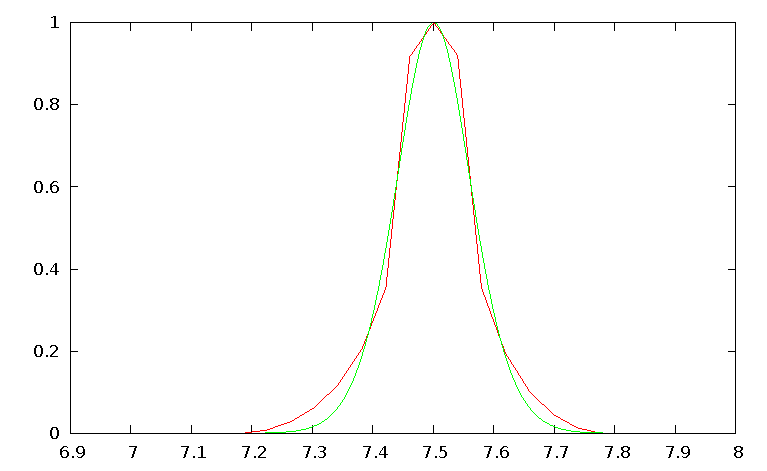
\includegraphics[scale=.62]{../static/model.pdf}
       
       Das Verfahren, das sich hier also anbietet ist, mit Hilfe der
       Spline-Suche ein vorläufiges Spektrum zu berechnen, und daraus
       einzelne Peaks auf einem vom Spektrum abhängendem Fenster zu isolieren.
       Anschließend Normiert man den Peak innerhalb des Fensters und minimiert
       die Funktion
       
       \begin{equation}
         \mathrm{ls}(x,a) = \sum_{i = 0}^{k} (m(x_i - x, a) - f_i)^2
       \end{equation}
       
       bezüglich $a$, wobei man für $x=x^{(0)}$ den Wert aus der Spline- 
       oder Akima-Suche
       benutzt. Auf diese Weise bekommt man den Wert $a^{(0)}$, mit dem man
       nun $\mathrm{ls}$ nach $x$ minimeiren kann und $x^{(1)}$ erhält.
       Falls $x^{(0)}$ nah
       am Peak-Mittelpunkt war, dann konvergiert dieses Verfahren seher schnell
       gegen den gesuchten Peak-Mittelpunkt $x_\mathrm{m}$.
       
       Die Grenzen dieses Verfahrens liegen natürlich genau dort, wo die
       Voraussetzung verletzt wird, dass die Peaks isoliert sind. 
       (Deswegen dann dieses Verfahren den Grundzustand des Kastenpotentials 
       ebenfalls nicht auflösen.)
       
   \subsection{Spektra}
		Wie schon in der oben angedeutet werde ich im Weiteren die gefundenen
		Energiewerte mit der Numerov-Approximation für die stationäre 
		Schrödingergleichung vergleichen.
		
%%%%%%%%%%%%%%%%%%%%%%%%%%%%%%%%%%%%%%%%%%%%%%%%%%%%%%%%%%%%%%%%%%%%%%%%%%%%%%%%
%%%%%%%%%%%%%%%%%%%%%%%%%%%%%%%%%%%%%%%%%%%%%%%%%%%%%%%%%%%%%%%%%%%%%%%%%%%%%%%%
%%%%%%%%%%%%%%%%%%%%%%%%%%%%%%%%%%%%%%%%%%%%%%%%%%%%%%%%%%%%%%%%%%%%%%%%%%%%%%%%
  	  \subsubsection{Asymetrischer Doppeltopf}
			  \includegraphics[scale=.62]{../data/simple/init}

  		  Das erste Potential ist ein einfaches Polynom 4. Ordnung, wobei die
    		Koeffizienten aus \cite{FFS} entnommen wurden. Leider konnte ich die
    		Ergebnisse von \cite{FFS} nicht für die genannten Parameter reproduzieren, 
  	  	die Energien stimmen jedoch für meine Konfiguration mit den gegebenen mehr 
  		  oder weniger überein. (Die Parameter aus \cite{FFS} sind offensichtlich falsch
    		ein $\tau = 5.7$ Entspricht einer maximalen simulierbaren Energie von
    		$\approx \pm0.551157$, die behaupteten Energien von $\approx-144$
  	  	können also niemals
    		aus einer Simulation mit diesen Parametern entstanden sein. Man erhält 
    		widerum ähnliche Werte wenn man sich um 4(!) Größenordnungen von
  	  	den agngegebenen Parametern entfernt, d.h. $\tau = \frac{5.7}{1000}$ und
  		  $\xi = \frac{0.825}{10}$).

  			Die Parameter werden an die Simulation mit Hilfe eines einfachen
	  		Lua-Skripts übergeben, in dem die Tabelle 
		  	\lstinline!config! definiert wird.
			  \lstinputlisting[language=Lua]{../presets/simple.lua}
  			Die einzelnen Variablen sind (Grau = optional)
			
	  		\begin{tabular}{ll}
		  		\lstinline!bins! & Anzahl der Stützstellen im Ort\\
			  	\lstinline!dt!   & einzelner Zeitschritt ($\tau$)\\
				  \lstinline!range!& das betrachtete \\
	  			                 & Ortsintervall $[-8,8]$\\
  				\lstinline!steps!& Zeitschritte zwischen \\
		  		                 & Korrelationsmessungen\\
			  	\lstinline!runs!& Anzahl Korrelationsmessungen\\
				  \rowcolor{lightgray}
  				\lstinline!vstep!& Zeitschritte zwischen Frames\\
	  			\rowcolor{lightgray}
		  		\lstinline!vframes!& Anzahl Frames\\
			  	\lstinline!potential(x)!& reelles Potential ($V(x)$)\\
				  \lstinline!psi(x)={u,v}!& Wellefunktion $\psi(x)=u+i v$\\
  				\rowcolor{lightgray}
	  			\lstinline!energie(k)!& exakte Energien $\epsilon_k$\\
		  		\lstinline!enrgrange!& betrachteten Energien:\\
          				 & Min.,Max.,\\
				           & Peak-Fenster(in Punkten),\\
				           & Suchschranke\\
  				\lstinline!output!& \\
	  			\lstinline!.dir!& Ausgabeverzeichnis\\
		  		\rowcolor{lightgray}
			  	\lstinline!.apsi!& Werte von $\psi(x,t=0)$\\
				  \rowcolor{lightgray}
  				\lstinline!.pot!& Werte von $V(x)$\\
	  			\rowcolor{lightgray}
		  		\lstinline!.corr!& Werte von $c(t)$\\
			  	\rowcolor{lightgray}
  				\lstinline!.dftcorr!& Werte von $\mathcal{F}[cw](\epsilon)$ \\
	  			\rowcolor{lightgray}
		  		\lstinline!.spectrum!& Peaks: direkte Suche \\
			  	\rowcolor{lightgray}
				  \lstinline!.numen!& Numerov Approximation \\
  				\rowcolor{lightgray}
	  			\lstinline!.splen!& Peaks: kubische Spline-Suche \\
		  		\rowcolor{lightgray}
			  	\lstinline!.aken!& Peaks: Akima-Suche \\
				  \rowcolor{lightgray}
  				\lstinline!.ccsen!& Peaks: nichtlineare Regression \\
	  		\end{tabular}
  
		  	\includegraphics[scale=.62]{../data/simple/corr}
    		\includegraphics[scale=.62]{../data/simple/spektrum}
    		
			  \begin{center}\input{../data/simple/spectrum.tex.inc}\end{center}
  			
	  		\includegraphics[scale=.62]{../data/simple/relen}
		  	
			  Wie man aus dem letzen Graphen entnehmen kann, wächst
  			der relative Fehler für größere Energien an.
  			
  			\paragraph*{Konvergeznverhalten}
  			  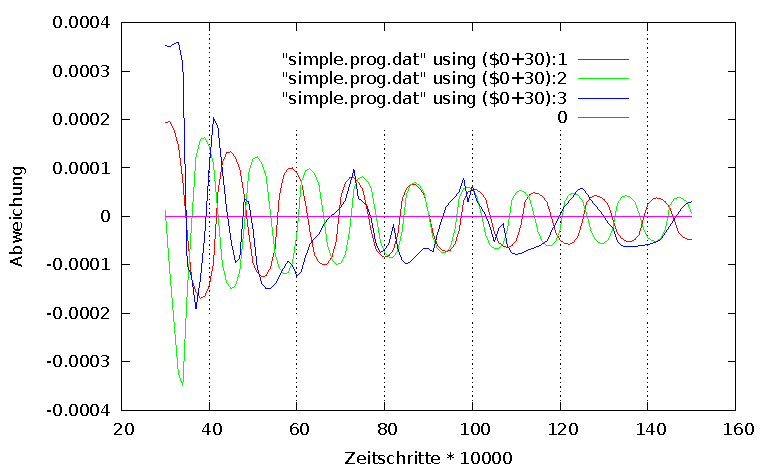
\includegraphics[scale=.62]{../static/simple_konv.pdf}
  			  Die Abweichung vom Numerov Wert wird mit der Anzahl der
  			  Zeitschritte kleiner, oszilliert aber
  			  mit einer vom Peak abhängender Frequenz.
			
%%%%%%%%%%%%%%%%%%%%%%%%%%%%%%%%%%%%%%%%%%%%%%%%%%%%%%%%%%%%%%%%%%%%%%%%%%%%%%%%
%%%%%%%%%%%%%%%%%%%%%%%%%%%%%%%%%%%%%%%%%%%%%%%%%%%%%%%%%%%%%%%%%%%%%%%%%%%%%%%%
%%%%%%%%%%%%%%%%%%%%%%%%%%%%%%%%%%%%%%%%%%%%%%%%%%%%%%%%%%%%%%%%%%%%%%%%%%%%%%%%			
  	  \subsubsection{Potentialkasten}
  			\includegraphics[scale=.62]{../data/square/init}
  			Als nächstes versuche ich bekannte Erbgebnisse für einen
	  		unendlich tiefen Potentialkasten näherungsweise mit einem
	  		endlich hohen  Potentialkasten zu approximieren.
	  		
	  		Die konfiguration für die Simulation lautet dementsprechend:
				\lstinputlisting[language=Lua]{../presets/square.lua}
				
		  	\includegraphics[scale=.62]{../data/square/corr}
    		\includegraphics[scale=.62]{../data/square/spektrum}
    		
			  \begin{center}\input{../data/square/spectrum.tex.inc}\end{center}
			  
	  		\includegraphics[scale=.62]{../data/square/relen}
	  		
	  		Der relative Fehler wird im Gegensatz zum vorgerigen Potential
	  		kleiner für größere Energien. Wie schon eingangs erwähnt, kann
	  		mein Verfahren die ersten drei Energien nicht auflösen. Die 
	  		Ergebnisse der reinen Spline-Suche bzw. Akima-Suche geben zwar einen
	  		Wert, dieser schwankt aber signifikant um den erwarteten.
	  		
  			\paragraph*{Konvergeznverhalten}
  			  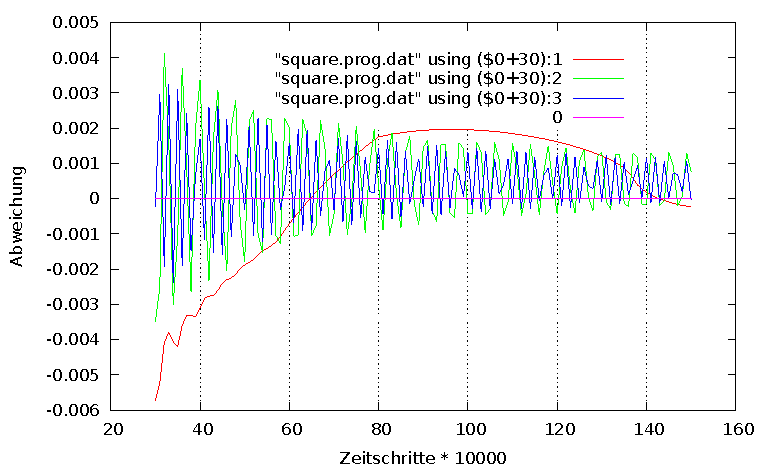
\includegraphics[scale=.62]{../static/square_konv.pdf}
%%%%%%%%%%%%%%%%%%%%%%%%%%%%%%%%%%%%%%%%%%%%%%%%%%%%%%%%%%%%%%%%%%%%%%%%%%%%%%%%
%%%%%%%%%%%%%%%%%%%%%%%%%%%%%%%%%%%%%%%%%%%%%%%%%%%%%%%%%%%%%%%%%%%%%%%%%%%%%%%%
%%%%%%%%%%%%%%%%%%%%%%%%%%%%%%%%%%%%%%%%%%%%%%%%%%%%%%%%%%%%%%%%%%%%%%%%%%%%%%%%	  		
	  		
%%%%%%%%%%%%%%%%%%%%%%%% FINAL>>> %%%%%%%%%%%%%%%%%%%%%%%%%%%%%%%%%%%%%%%%%%%%%%
      \subsubsection*{Harmonischer Oszillator}
  			\includegraphics[scale=.62]{../data/harmosca/init}

        Als letrztes Potential betrachte ich den Harmonischen Oszillator, 
        da für ihn die Exakte werte bekannt sind.  In der Konfugurationsdatei
        werden diese mit der Funktion \verb!energy! festegelgt:
  			
			  \lstinputlisting[language=Lua]{../presets/harmosca.lua}
		
			  \begin{center}\input{../data/harmosca/spectrum.tex.inc}\end{center}
			  
		  	\includegraphics[scale=.62]{../data/harmosca/corr}
    		\includegraphics[scale=.62]{../data/harmosca/spektrum}
			  
	  		\includegraphics[scale=.62]{../data/harmosca/relen}
	  		
	  		Auch bei diesem Potential verringert sich der relative Fehler 
	  		für größere Energiewerte.
	  		
  			\paragraph*{Konvergeznverhalten}
  			  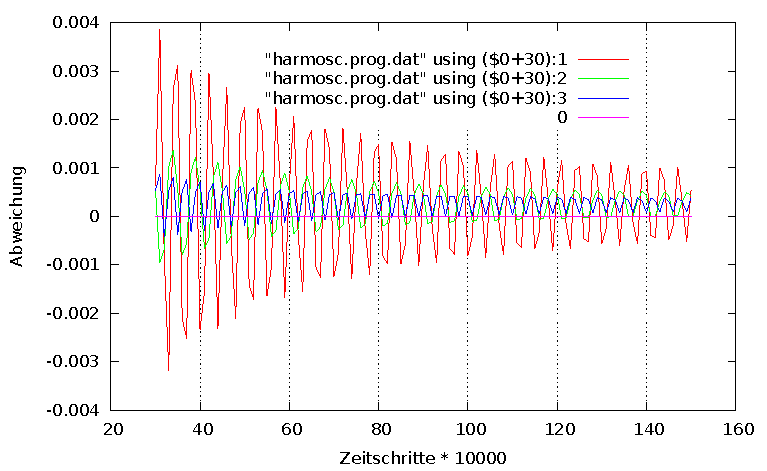
\includegraphics[scale=.62]{../static/harmosc_konv.pdf}
  			  Die Abweichung vom Numerov Wert wird auch für dieses Potential
  			  kleiner und auch hier ist eine deutliche Überlagerung
  		    mit einer Schwingung zu sehen.
  		    
	\section{Fazit}
		Wie man aus der betrachtung der Spektra entnehmen kann, erlaubt die
		Autokorrelations-Methode immer die grobe Bestimmung eines Spektrums.
		Auch behält dieses Spektrum bei kleinen Veränderungen der 
		Simulationsparamter seine Form.
		
		
		Für genaue Approximation von des Spektrums eignet sich diese Verfahren
		leider nicht: Das Konvergenzverhalten ist so, dass jeder Peaks
		mit einer eigenen Frequenz oszilliert, die man bei der Suche nicht 
		berücksichtigen kann, da man sie apriori nicht wissen kann.
		
	\section{Quellcode}
	  Der Quellkode ist unter
	  \url{https://github.com/xaberus/project3}
	  veröffentlicht und lässt sich mit
	  \verb!git clone git://github.com/xaberus/project3.git! herunterladen.
			
%%%%%%%%%%%%%%%%%%%%%%%%%%%%%%%%%%%%%%%%%%%%%%%%%%%%%%%%%%%%%%%%%%%%%%%%%%%%%%%%

	\begin{thebibliography}{}
		\bibitem[FFS]{FFS}
			\newblock{M.D Feit, J.A Fleck Jr., A Steiger}
			\newblock{\em{Solution of the Schrödinger equation by a spectral method}}
			\newblock{\url{http://dx.doi.org/10.1016/0021-9991(82)90091-2}}
		\bibitem[FMF]{FMF}
			\newblock{J. A. Fleck, J. R. Morris and M. D. Feit}
			\newblock{\em{
				Time-dependent propagation of high energy laser beams through the atmosphere}}
			\newblock{\url{http://dx.doi.org/10.1007/BF00896333}}
		\bibitem[MA]{MA}
			\newblock{Mrinal Mandal, Amir Asif}
			\newblock{\em{Continuous and Discrete Time Signals and Systems}}
			\newblock{Kap.12.1}
			\newblock{\url{
				http://www.cambridge.org/resources/
				0521854555/4421_Chapter\%2012\%20-\%20Discrete\%20Fourier\%20transform.pdf}}
		\bibitem[SAPS]{SAPS}
			\newblock{Girish Keshav Palshikar}
			\newblock{\em{Simple Algorithms for Peak Detection in Time-Series}}
			\newblock{\url{
			http://www.tcs-trddc.com/trddc_website/pdf/SRL/Palshikar_SAPDTS_2009.pdf}}
	\end{thebibliography}
\end{document}
